% !TeX encoding = UTF-8
% !TeX TS-program = latexmk
% Mathematical Programming: An Introduction to Optimization
% Faithful reconstruction of source PDF pages 1--80, updated to the
% Fall 2026 syllabus (course information, objectives, learning outcomes,
% teaching assistants, and textbook).
% See mathematical-programming-2026-2027-corrections.md for every change.

\PassOptionsToPackage{cmyk}{xcolor}
\documentclass[aspectratio=169,hyperref,UTF8,CJK]{beamer}

\makeatletter
\newcommand{\beamer@scu@fontextend}{%
  \setsansfont{Latin Modern Sans}%
  \setmonofont{Latin Modern Mono}%
  \setCJKsansfont{PingFang SC}%
}
\makeatother

\usetheme[
  ColorDisplay=JXred,
  BlockDisplay=followtheme,
  CodeTheme=listing,
  LanguageMode=en,
  Miniframes=follow,
  NavigationTool=1-2-3,
  FontTheme=Custom,
  MathFont=LM,
  BIBMode=none,
  ContentMuticols=false,
  Background=SCU-Full
]{scu}

\usepackage{array}
\usepackage{booktabs}
\usepackage{mathtools}
\usepackage{multirow}
\usepackage{tabularx}

\newcommand{\R}{\mathbb{R}}
\newcommand{\trans}{\mathsf{T}}
\newcommand{\vect}[1]{\boldsymbol{#1}}

\title[Introduction to Optimization]{Introduction to Optimization}
\subtitle{Mathematical Programming}
\author[Changxi Wang]{Changxi Wang}
\institute{Sichuan University-Pittsburgh Institute\\Chengdu, China}
\date{2026--2027 Academic Year}

% Disable the theme's extra subsection-outline pages so source page n remains
% output page n (automatic title page plus 79 content frames).
\AtBeginSubsection[]{}

\begin{document}

% Source PDF page 001: title page. Instructor and academic year updated.

\section{Introduction}
\subsection{Course Information}

% Source PDF page 002. Updated to the Fall 2026 syllabus (course logistics,
% textbook, reference, and grade breakdown).
\begin{frame}{About the Course}
  \footnotesize
  \begin{itemize}
    \item \textbf{Course}: MATH 1101 --- An Introduction to Optimization
    \item \textbf{Instructor}: Changxi Wang (Office: SCUPI N403, \url{changxi.wang@scai-ji.cn}, Office Hours: Tue 8:15--11:00)
    \item \textbf{Lecture}: Tuesday 19:20--21:55, SCUPI Building S204
    \item \textbf{Recitation}: One 45-minute recitation per week
    \item \textbf{Performance Assessment}:
      \begin{enumerate}
        \item Attendance (10\%)
        \item Quiz (10\%)
        \item Homework (15\%)
        \item Mid-term Exam (30\%)
        \item Final Examination (35\%)
      \end{enumerate}
  \end{itemize}
\end{frame}

% Added per Fall 2026 syllabus: textbook details.
\begin{frame}{Textbook}
  \small
  \begin{columns}[T,onlytextwidth]
    \begin{column}{0.36\textwidth}
      \centering
      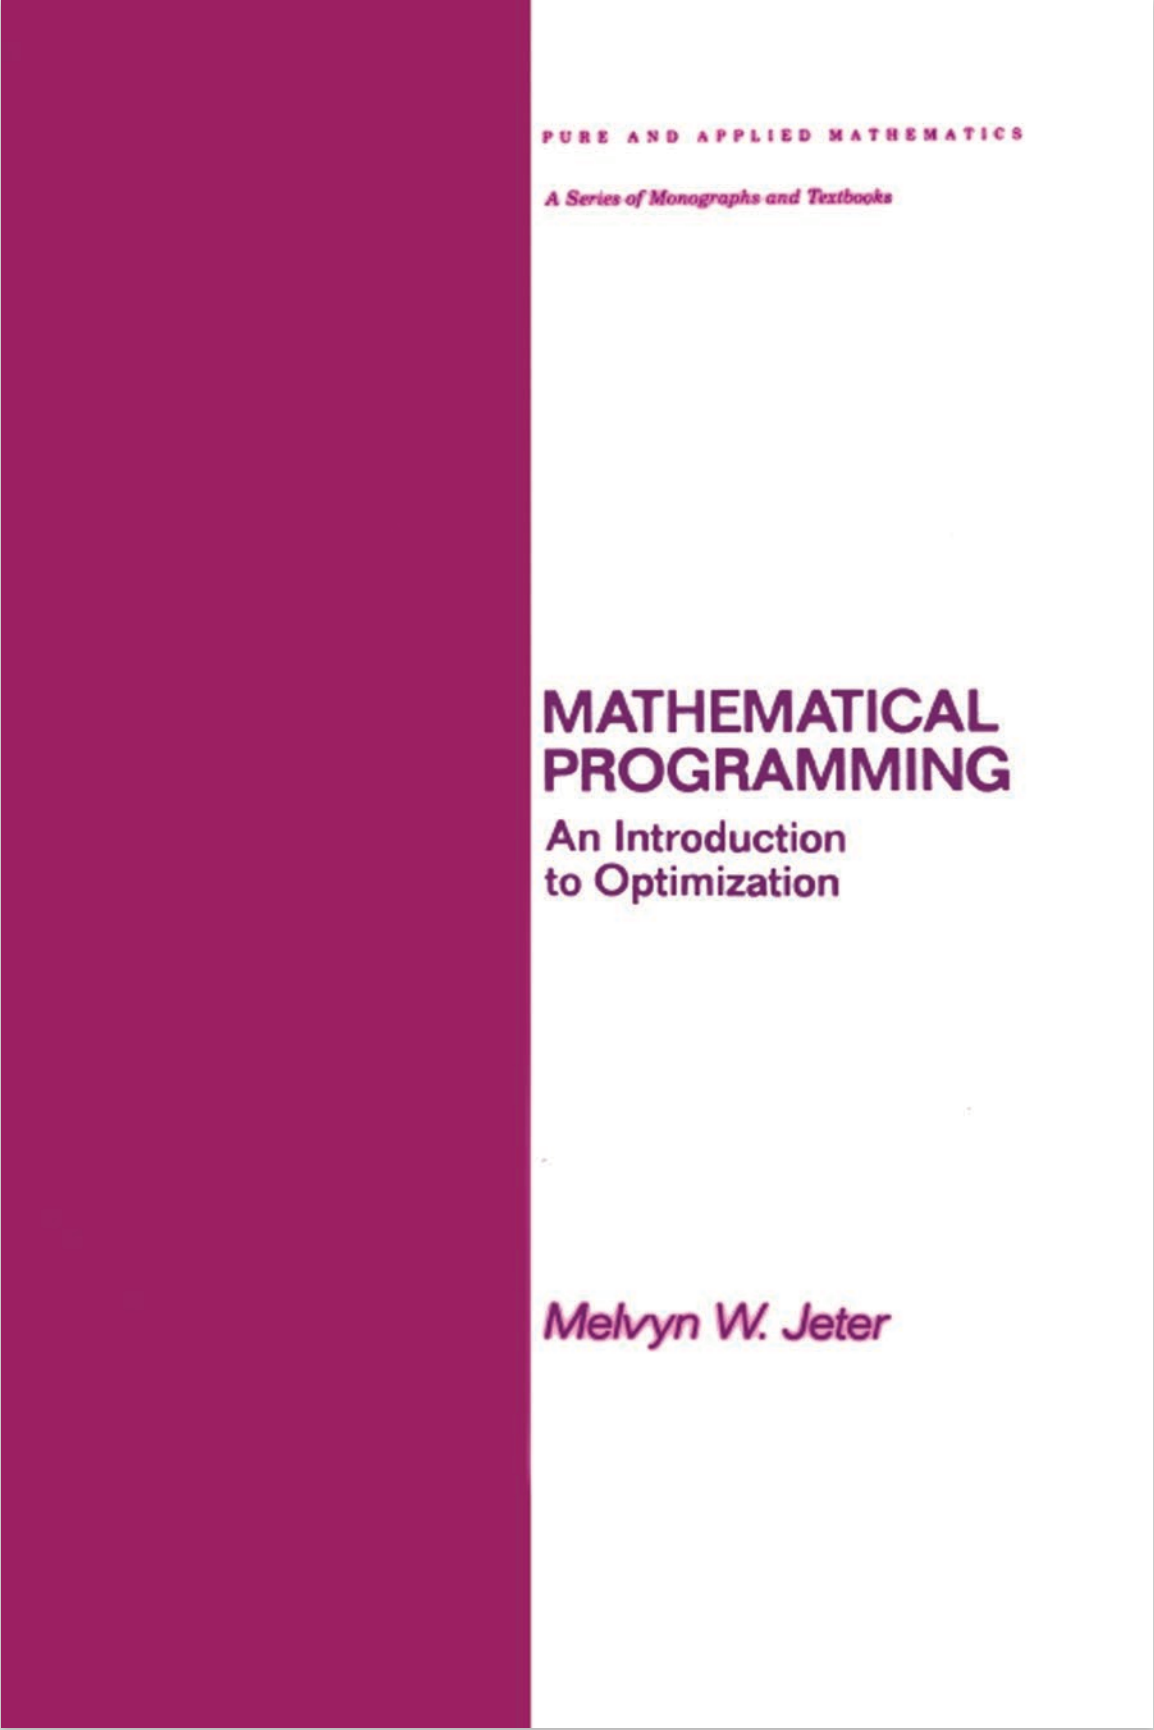
\includegraphics[width=\linewidth,height=0.70\textheight,keepaspectratio]{figures/Mathematical_Programming.png}
    \end{column}
    \begin{column}{0.60\textwidth}
      \begin{itemize}
        \item \textbf{Title}: \emph{Mathematical Programming: An Introduction to Optimization}
        \item \textbf{Author}: Melvyn W. Jeter
        \item \textbf{Publisher}: CRC Press, 1986
        \item \textbf{Preview}: \url{https://api.pageplace.de/preview/DT0400.9781351433136_A37628884/preview-9781351433136_A37628884.pdf}
        \item \textbf{Reference}: \emph{Convex Optimization}, by Stephen Boyd and Lieven Vandenberghe, Cambridge University Press
      \end{itemize}
    \end{column}
  \end{columns}
\end{frame}

% Added per Fall 2026 syllabus: course objectives.
\begin{frame}{Course Objectives}
  \small
  By the end of this course, students will be able to:
  \begin{enumerate}
    \item Recognize and formulate optimization problems in diverse domains.
    \item Understand the mathematical foundations of optimization, including convex sets, convex functions, and related function properties.
    \item Apply optimality conditions (first-order, second-order, KKT) to analyze problems.
    \item Use duality theory to interpret and solve optimization problems.
    \item Implement and analyze basic optimization algorithms, including gradient descent, Newton's method, and interior-point methods.
    \item Appreciate the applications of optimization in engineering, data science, and beyond.
  \end{enumerate}
\end{frame}

% Added per Fall 2026 syllabus: learning outcomes.
\begin{frame}{Learning Outcomes}
  \small
  \begin{enumerate}
    \item Formulate real-world problems as mathematical optimization problems.
    \item Classify problems as convex, nonconvex, linear, or nonlinear.
    \item Apply convex analysis tools to study problem feasibility and structure.
    \item Derive and interpret optimality conditions.
    \item Use duality theory to analyze sensitivity and design algorithms.
    \item Implement and analyze gradient-based and Newton-type optimization algorithms.
    \item Assess trade-offs between accuracy, computational complexity, and convergence rate.
  \end{enumerate}
\end{frame}

% Added per Fall 2026 syllabus: material covered (weeks 1--9).
\begin{frame}{Material Covered (Weeks 1--9)}
  \scriptsize
  \begin{tabularx}{\textwidth}{@{}c l X@{}}
    \toprule
    Week & Date & Content \\
    \midrule
    1 & Sep 3 & Course overview, basic optimization formulation, LP definition, and modeling examples (manufacturing, assignment, portfolio), Global/local optima. \\
    2 & Sep 10 & Topology basics, sensitivity (post-optimal) analysis, parametric programming, and model stability, Matrices, vectors. \\
    3 & Sep 17 & Subspaces, bases, matrix operations, inverses, and elementary row operations, Gaussian elimination and LU decomposition, affine sets. \\
    4 & Sep 24 & Convex sets, convex hulls, and cones, Hyperplanes, polytopes, extreme points. \\
    5 & Oct 1 & LP standard forms, convexity of the feasible set, Finite Basis Theorem, optimality at extreme points, vertex enumeration. \\
    6 & Oct 8 & Basic feasible solutions, the simplex tableau, pivoting rules, and optimality conditions. \\
    7 & Oct 15 & Mid-term Exam. \\
    8 & Oct 22 & Full worked examples, including unbounded and multiple-optimum cases. \\
    9 & Oct 29 & Big-M/two-phase method with artificial variables and initial tableau construction. \\
    \bottomrule
  \end{tabularx}
\end{frame}

% Added per Fall 2026 syllabus: material covered (weeks 10--18).
\begin{frame}{Material Covered (Weeks 10--18)}
  \scriptsize
  \begin{tabularx}{\textwidth}{@{}c l X@{}}
    \toprule
    Week & Date & Content \\
    \midrule
    10 & Nov 5 & Advanced cases: degeneracy, infeasibility, and multiple optimal solutions. \\
    11 & Nov 12 & Dual problem construction, weak/strong duality, and the fundamental duality theorem. \\
    12 & Nov 19 & General dual forms, symmetric duals, economic interpretation, and complementary slackness. \\
    13 & Nov 26 & Convex/concave definitions, quadratic forms, definiteness, and level sets. \\
    14 & Dec 3 & Epigraph, one-variable convexity, gradients, directional derivatives, Taylor's theorem, and multivariable convexity. \\
    15 & Dec 10 & Optimality conditions for convex problems, quasiconvex functions, star-shaped sets. \\
    16 & Dec 17 & First-order necessary conditions, nonnegative variables, and Lagrange multipliers with examples. \\
    17 & Dec 24 & Inequality constraints, Kuhn-Tucker (KKT) conditions and theorems, final review. \\
    18 & Dec 25 (TBD) & Final Exam. \\
    \bottomrule
  \end{tabularx}
\end{frame}

% Source PDF page 003. Updated to the Fall 2026 teaching assistants.
\begin{frame}{Teaching Assistants}
  \small
  \begin{columns}[T,onlytextwidth]
    \begin{column}{0.55\textwidth}
      \begin{itemize}
        \item Yifan Lyu 吕一凡
          \begin{itemize}
            \item Email: \url{lyuyifan@stu.scu.edu.cn}
          \end{itemize}
        \item Guanmeng Xian 贤冠萌
          \begin{itemize}
            \item Email: \url{xianguanmeng@stu.scu.edu.cn}
          \end{itemize}
      \end{itemize}
    \end{column}
    \begin{column}{0.41\textwidth}
      \begin{itemize}
        \item Office: SCUPI Building N407
        \item Office Hours: Tuesday 8:15--11:00
        \item QQ Group: 1108310197
      \end{itemize}
    \end{column}
  \end{columns}
\end{frame}

% Source PDF page 004
\begin{frame}{Introduction}
  \begin{itemize}
    \item An introduction to optimization for students with background of linear algebra, calculus, and multivariable calculus
    \item Optimization is used everywhere nowadays with growing importance
    \item Applications:
      \begin{itemize}
        \item Economic analysis
        \item Management
        \item Engineering technology
        \item Military operations
        \item etc
      \end{itemize}
  \end{itemize}
\end{frame}

% Source PDF page 005
\begin{frame}{Examples}
  \centering
  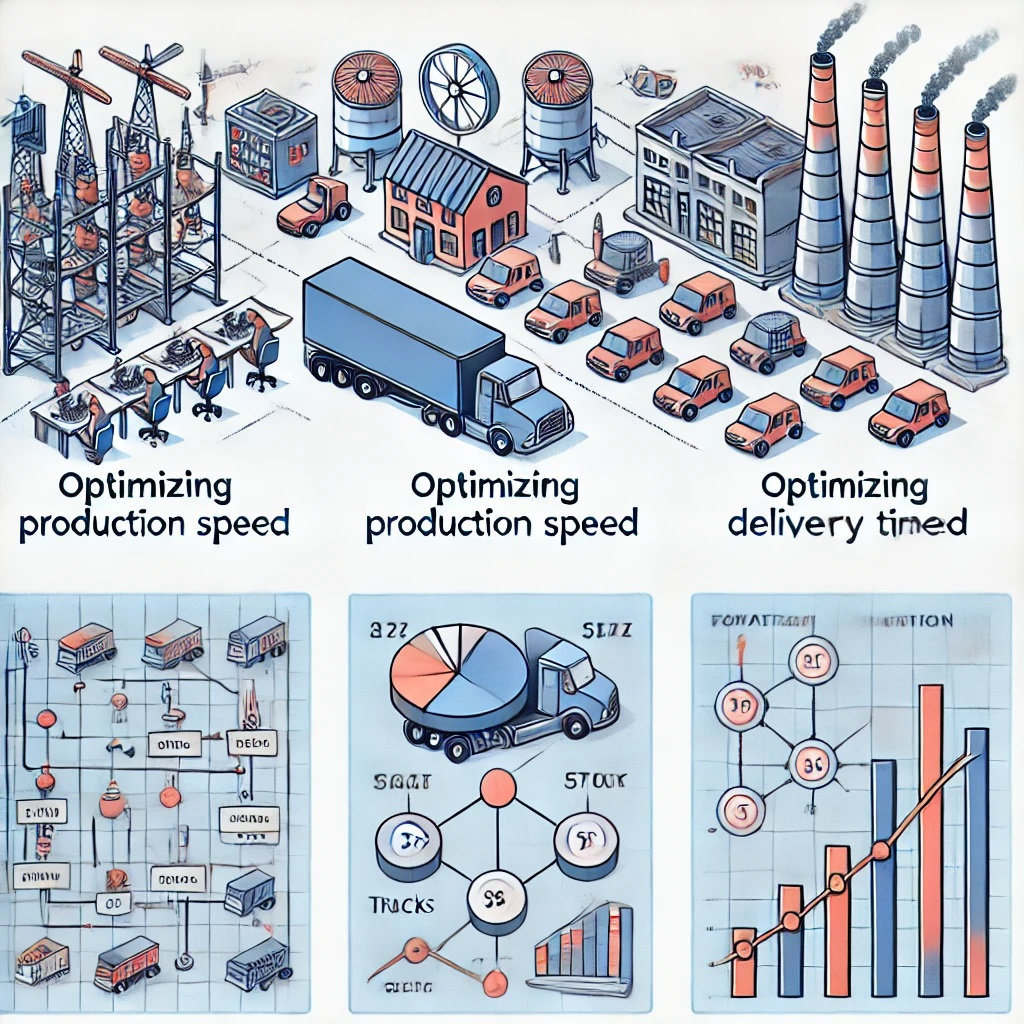
\includegraphics[width=0.77\linewidth,height=0.76\textheight,keepaspectratio]{figures/mp-2026/p005-optimization-manufacturing.jpg}
\end{frame}

% Source PDF page 006
\begin{frame}{Examples}
  \centering
  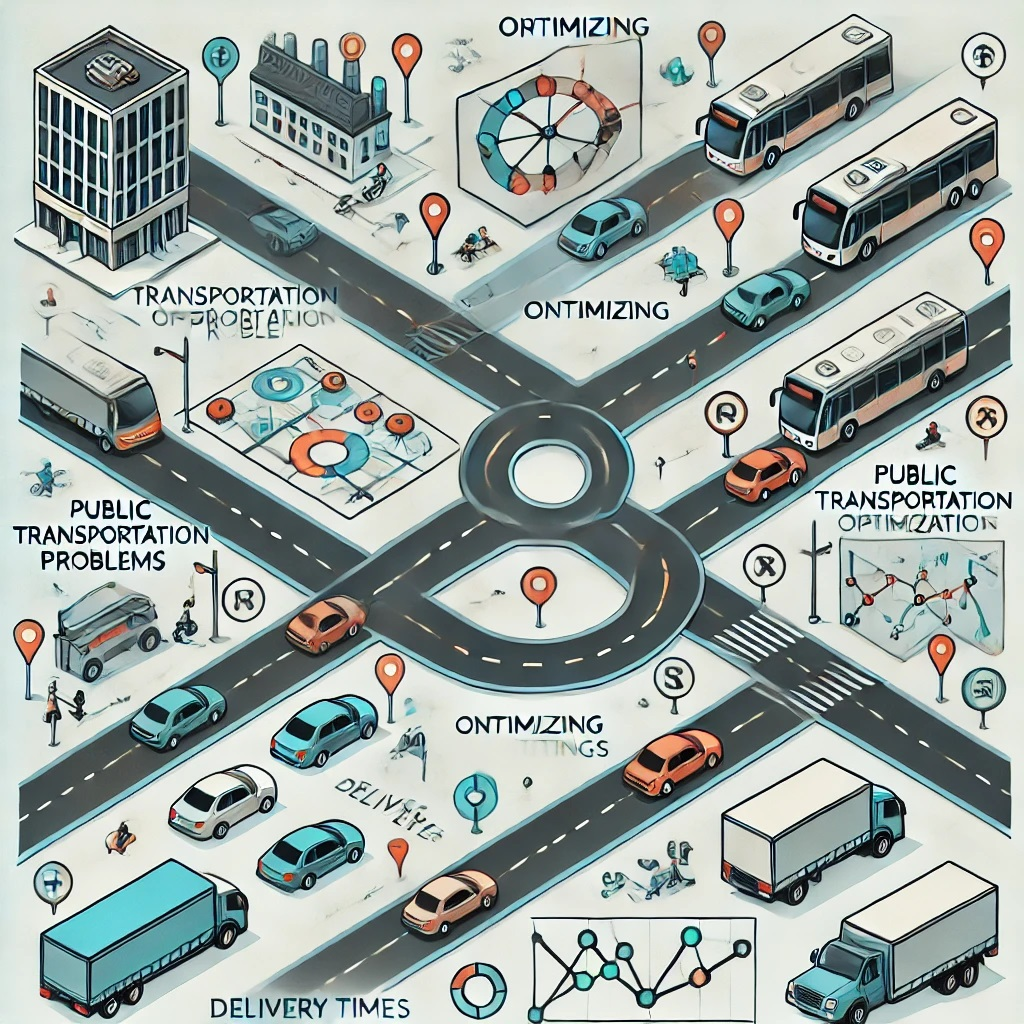
\includegraphics[width=0.77\linewidth,height=0.76\textheight,keepaspectratio]{figures/mp-2026/p006-optimization-transportation.jpg}
\end{frame}

\section{Mathematical Programming Problems}
\subsection{Basic Models}

% Source PDF page 007
\begin{frame}{The Basic Mathematical Programming Problem}
  \small
  \begin{itemize}
    \item Definition:
      \begin{align}
        \min\ f(x_1,x_2,\ldots,x_n)\quad &\text{or}\quad \max\ f(x_1,x_2,\ldots,x_n) \tag{1}\\
        \text{s.t.}\quad &(x_1,x_2,\ldots,x_n)\in\Omega \tag{2}
      \end{align}
      where
      \begin{itemize}
        \item $f(x_1,x_2,\ldots,x_n)$ in (1) is the cost (objective) function.
        \item $\Omega$ in (2) is the set of feasible solutions.
      \end{itemize}
    \item Unconstrained problem: $\Omega=\{(x_1,\ldots,x_n):x_i\in\R\}$.
    \item Constrained problem: $\Omega$ is a proper subset of $\{(x_1,\ldots,x_n):x_i\in\R\}$.
  \end{itemize}
\end{frame}

% Source PDF page 008
\begin{frame}{Linear Programming Problem}
  \footnotesize
  \begin{itemize}
    \item Linear cost function:
      \begin{equation}\tag{3}
        f(x_1,\ldots,x_n)=c_1x_1+\ldots+c_nx_n,
      \end{equation}
      where $c_1,\ldots,c_n$ are real constants. $c_i$ is called the cost coefficient of the variable $x_i$.
    \item An equality constraint:
      \begin{equation}\tag{4}
        a_1x_1+\ldots+a_nx_n=b,
      \end{equation}
      where $a_1,\ldots,a_n$ are real constants.
    \item A linear inequality constraint:
      \begin{equation}\tag{5}
        a_1x_1+\ldots+a_nx_n\gtreqless b,
      \end{equation}
    \item A problem that is NOT linear programming: nonlinear programming problem.
    \item Generally, linear programming problems are easier than nonlinear ones.
  \end{itemize}
\end{frame}

\subsection{Examples}

% Source PDF page 009
\begin{frame}{Example 1}
  \small
  \begin{itemize}
    \item A manufacturer produces $n$ products $P_1,P_2,\ldots,P_n$ from $m$ raw materials $M_1,\ldots,M_m$. The amount of each raw material required for each product:
      \begin{center}
        \begin{tabular}{c|cccc}
          & $P_1$ & $P_2$ & $\cdots$ & $P_n$\\ \hline
          $M_1$ & $a_{1,1}$ & $a_{1,2}$ & $\cdots$ & $a_{1,n}$\\
          $M_2$ & $a_{2,1}$ & $a_{2,2}$ & $\cdots$ & $a_{2,n}$\\
          $\vdots$ & $\vdots$ & $\vdots$ & $\ddots$ & $\vdots$\\
          $M_m$ & $a_{m,1}$ & $a_{m,2}$ & $\cdots$ & $a_{m,n}$
        \end{tabular}
      \end{center}
    \item Available: $b_i$ units of $M_i$, $\forall i=1,\ldots,m$.
    \item Revenue: $c_j$ dollars for each unit of $P_j$ sold.
    \item Question: Desire to maximize the total daily revenue.
  \end{itemize}
\end{frame}

% Source PDF page 010
\begin{frame}{Example 1}
  \begin{itemize}
    \item $x_j$: \# of product $P_j$ that has been produced.
    \item $a_{i,j}x_j$: \# of material $M_i$ used to produce $x_j$ units of $P_j$.
    \item \# of the daily revenue:
      \begin{equation}\tag{6}
        c_1x_1+\ldots+c_nx_n
      \end{equation}
    \item \# of material $M_i$ consumed in total:
      \begin{equation}\tag{7}
        a_{i,1}x_1+\ldots+a_{i,n}x_n\le b_i,
      \end{equation}
  \end{itemize}
\end{frame}

% Source PDF page 011
\begin{frame}{Example 1}
  \small
  \begin{itemize}
    \item The cost function:
      \begin{equation}\tag{8}
        \max_{x_j,\,\forall j\in[1,n]}\{c_1x_1+\ldots+c_nx_n\}
      \end{equation}
      subject to
      \begin{equation}\tag{9}
      \begin{aligned}
        a_{1,1}x_1+a_{1,2}x_2+\ldots+a_{1,n}x_n&\le b_1,\\
        a_{2,1}x_1+a_{2,2}x_2+\ldots+a_{2,n}x_n&\le b_2,\\
        &\vdots\\
        a_{m,1}x_1+a_{m,2}x_2+\ldots+a_{m,n}x_n&\le b_m,\\
        x_1\ge0,\ x_2\ge0,\ldots,\ x_n&\ge0.
      \end{aligned}
      \end{equation}
  \end{itemize}
\end{frame}

% Source PDF page 012
\begin{frame}{Example 1}
  \small
  \begin{itemize}
    \item Continuous variable: allowed to take on all fractional as well as integral values within its range of variation
    \item Discrete variable: must take on values from a discrete set of values
    \item Slack variable: inequality can be converted to an equality constraint by adding a non-negative variable
      \begin{itemize}
        \item Take (9) for example:
          \begin{equation*}
            a_{1,1}x_1+\ldots+a_{1,n}x_n+x_{n+1}=b_1,
          \end{equation*}
          $x_{n+1}$: Slack variable, assigned a cost coefficient of $c_{n+1}=0$
      \end{itemize}
  \end{itemize}
\end{frame}

% Source PDF page 013
\begin{frame}{Example 1}
  \footnotesize
  \begin{itemize}
    \item The cost function (8) can be reformulated as
      \begin{equation*}
        \max_{x_j,\,\forall j\in[1,n+m]}
        \underbrace{\{c_1x_1+\ldots+c_nx_n+c_{n+1}x_{n+1}+\ldots+c_{n+m}x_{n+m}\}}
        _{=\max_{x_j,\,\forall j\in[1,n]}\{c_1x_1+\ldots+c_nx_n\}}
      \end{equation*}
      subject to
      \begin{align*}
        a_{1,1}x_1+a_{1,2}x_2+\ldots+a_{1,n}x_n+x_{n+1}&=b_1,\\
        a_{2,1}x_1+a_{2,2}x_2+\ldots+a_{2,n}x_n+x_{n+2}&=b_2,\\
        &\vdots\\
        a_{m,1}x_1+a_{m,2}x_2+\ldots+a_{m,n}x_n+x_{n+m}&=b_m,\\
        x_1\ge0,\ldots,x_n\ge0,\quad x_{n+1}\ge0,\ldots,x_{n+m}&\ge0.
      \end{align*}
  \end{itemize}
\end{frame}

% Source PDF page 014
\begin{frame}{Example 2}
  \begin{itemize}
    \item 4 salesmen + 4 sales districts
    \item The sales productivity ratings for each salesman $S_i$ in each sales districts $D_j$:
      \begin{center}
        \begin{tabular}{c|rrrr}
          & $D_1$ & $D_2$ & $D_3$ & $D_4$\\ \hline
          $S_1$ & 5 & 10 & 8 & 2\\
          $S_2$ & 3 & 4 & 2 & 6\\
          $S_3$ & 9 & 5 & 4 & 5\\
          $S_4$ & 5 & 5 & 6 & 4
        \end{tabular}
      \end{center}
    \item Question: Determine the best assignment of salesman to sales districts.
  \end{itemize}
\end{frame}

% Source PDF page 015
\begin{frame}{Example 2}
  \footnotesize
  \begin{itemize}
    \item Define
      \begin{equation}\tag{10}
        x_{i,j}=\begin{cases}1,&\text{if $S_i$ assigned to $D_j$},\\0,&\text{otherwise.}\end{cases}
      \end{equation}
    \item The value of an assignment:
      \begin{align*}
        f(x_{i,j})={}&5x_{1,1}+10x_{1,2}+8x_{1,3}+2x_{1,4}+3x_{2,1}+4x_{2,2}+2x_{2,3}+6x_{2,4}\\
        &+9x_{3,1}+5x_{3,2}+4x_{3,3}+5x_{3,4}+5x_{4,1}+5x_{4,2}+6x_{4,3}+4x_{4,4}.
      \end{align*}
    \item Each salesman must be assigned to exactly one district:
      \begin{equation}\tag{11}
        \sum_{j=1}^{4}x_{i,j}=1,\qquad \forall i.
      \end{equation}
    \item Each district is assigned exactly one salesman:
      \begin{equation}\tag{12}
        \sum_{i=1}^{4}x_{i,j}=1,\qquad \forall j.
      \end{equation}
  \end{itemize}
\end{frame}

% Source PDF page 016
\begin{frame}{Example 2}
  \begin{itemize}
    \item Problem:
      \begin{equation*}
        \max_{\forall i,j}\{f(x_{i,j})\}
      \end{equation*}
      subject to
      \begin{align*}
        x_{i,1}+x_{i,2}+x_{i,3}+x_{i,4}&=1, &&\forall i,\\
        x_{1,j}+x_{2,j}+x_{3,j}+x_{4,j}&=1, &&\forall j,\\
        0\le x_{i,j}&\le1, &&\forall i,j.
      \end{align*}
  \end{itemize}
\end{frame}

% Source PDF page 017
\begin{frame}{Example 3}
  \small
  \begin{itemize}
    \item A flour company has 3 production lines which can produce A and B. The number of ten pound sacks of flour which can be produced daily by each of the production lines is summarized in the following table:
      \begin{center}
        \begin{tabular}{c|rrr}
          & $L_1$ & $L_2$ & $L_3$\\ \hline
          A & 15000 & 10000 & 12000\\
          B & 12000 & 13500 & 14500
        \end{tabular}
      \end{center}
    \item Question: Produce as many ten pound bags of flour of brands A and B as possible.
  \end{itemize}
\end{frame}

% Source PDF page 018
\begin{frame}{Example 3}
  \small
  \begin{itemize}
    \item Define
      \begin{equation*}
        x_i=\begin{cases}1,&\text{if $L_i$ assigned to A},\\0,&\text{otherwise,}\end{cases}
        \qquad
        w_i=\begin{cases}1,&\text{if $L_i$ assigned to B},\\0,&\text{otherwise.}\end{cases}
      \end{equation*}
    \item A production line cannot be assigned to both products:
      \begin{equation*}
        x_1w_1=0,\quad x_2w_2=0,\quad x_3w_3=0.
      \end{equation*}
    \item All variables are non-negative
  \end{itemize}
\end{frame}

% Source PDF page 019
\begin{frame}{Example 3}
  \begin{itemize}
    \item The above two constraints can be compressed into one:
      \begin{equation}\tag{13}
        \sum_{i=1}^{3}x_iw_i=x_1w_1+x_2w_2+x_3w_3=0.
      \end{equation}
    \item To insure that each production line is assigned to a job:
      \begin{align*}
        x_1+w_1&=1,\\
        x_2+w_2&=1,\\
        x_3+w_3&=1.
      \end{align*}
  \end{itemize}
\end{frame}

% Source PDF page 020
\begin{frame}{Example 3}
  \small
  \begin{itemize}
    \item A nonlinear programming problem:
      \begin{equation*}
        \max_{\forall x_i,w_j}\{15000x_1+10000x_2+12000x_3+12000w_1+13500w_2+14500w_3\}
      \end{equation*}
      subject to
      \begin{align*}
        x_1+w_1&=1,\\
        x_2+w_2&=1,\\
        x_3+w_3&=1,\\
        \sum_{i=1}^{3}x_iw_i&=0,\quad\text{(complementary constraint)}\\
        0\le x_i\le1,\quad 0\le w_i&\le1,\quad\forall i.
      \end{align*}
  \end{itemize}
\end{frame}

% Source PDF page 021
\begin{frame}{Example 4}
  \small
  \begin{itemize}
    \item Quadratic (nonlinear) programming problem:
      \begin{equation*}
        \max_{\forall i,j}\left\{c_1x_1+\ldots+c_nx_n+\sum_{i=1}^{n}\sum_{j=1}^{n}b_{ij}x_ix_j\right\}
      \end{equation*}
      subject to
      \begin{align*}
        a_{11}x_1+a_{12}x_2+\ldots+a_{1n}x_n&=b_1,\\
        a_{21}x_1+a_{22}x_2+\ldots+a_{2n}x_n&=b_2,\\
        &\vdots\\
        a_{m1}x_1+a_{m2}x_2+\ldots+a_{mn}x_n&=b_m,\\
        x_1\ge0,\quad x_2\ge0,\ldots,\quad x_n&\ge0.
      \end{align*}
  \end{itemize}
\end{frame}

% Source PDF page 022
\begin{frame}{Example 4}
  \small
  \begin{itemize}
    \item The portfolio selection problem:
      \begin{equation*}
        \max_{\forall i,j}\left\{c_1x_1+\ldots+c_nx_n-\sum_{i=1}^{n}\sum_{j=1}^{n}b_{i,j}x_ix_j\right\}
      \end{equation*}
      subject to
      \begin{align*}
        x_1+\ldots+x_n&=1,\\
        x_1\ge0,\ldots,x_n&\ge0.
      \end{align*}
    \item $x_i$: investment
    \item $c_i$: expected rate of return
    \item $\sum_{i=1}^{n}\sum_{j=1}^{n}b_{i,j}x_ix_j$: risk of investment
  \end{itemize}
\end{frame}

\subsection{Solutions, Topology, and Sensitivity}

% Source PDF page 023
\begin{frame}{Global And Local Solutions}
  \begin{itemize}
    \item Standard Euclidean distance:
      \begin{equation*}
        \lVert\vect{x}-\bar{\vect{x}}\rVert=\sqrt{\sum_{i=1}^{n}(x_i-\bar{x}_i)^2}
      \end{equation*}
    \item Neighborhood of $\bar{\vect{x}}$:
      \begin{equation*}
        N_{\varepsilon}(\bar{\vect{x}})=\{\vect{x}:\lVert\vect{x}-\bar{\vect{x}}\rVert<\varepsilon\}
      \end{equation*}
      where $\varepsilon$ is a positive real number.
  \end{itemize}
\end{frame}

% Source PDF page 024. Strict-minimum comparison point corrected; irrelevant
% existential epsilon removed from the two global definitions.
\begin{frame}{Global And Local Solutions}
  \small
  \begin{itemize}
    \item Local minimum (at $\bar{\vect{x}}\in\Omega$):
      \begin{equation*}
        \exists\varepsilon>0,\ \text{such that }f(\bar{\vect{x}})\le f(\vect{x}),\quad
        \forall\vect{x}\in\Omega\cap N_{\varepsilon}(\bar{\vect{x}}).
      \end{equation*}
    \item Strict local minimum:
      \begin{equation*}
        \exists\varepsilon>0,\ \text{such that }f(\bar{\vect{x}})<f(\vect{x}),\quad
        \forall\vect{x}\in(\Omega\cap N_{\varepsilon}(\bar{\vect{x}}))\setminus\{\bar{\vect{x}}\}.
      \end{equation*}
    \item Global minimum:
      \begin{equation*}
         \exists\varepsilon>0,\ \text{such that }f(\bar{\vect{x}})\le f(\vect{x}),\quad\forall\vect{x}\in\Omega.
      \end{equation*}
    \item Strict global minimum:
      \begin{equation*}
         \exists\varepsilon>0,\ \text{such that }f(\bar{\vect{x}})<f(\vect{x}),\quad\forall\vect{x}\in\Omega\setminus\{\bar{\vect{x}}\}.
      \end{equation*}
  \end{itemize}
\end{frame}

% Source PDF page 025
\begin{frame}{Topology Concepts}
  \small
  \begin{itemize}
    \item The interior of $\Omega$:
      \begin{equation*}
        \operatorname{Int}(\Omega)=\{\vect{x}\in\Omega:N_{\varepsilon}(\vect{x})\subseteq\Omega\text{ for some }\varepsilon>0\}.
      \end{equation*}
    \item $\Omega$ is open if $\Omega=\operatorname{Int}(\Omega)$, i.e., every point of $\Omega$ is an interior point
    \item The exterior of $\Omega$:
      \begin{equation*}
        \operatorname{Ext}(\Omega)=\{\vect{x}:N_{\varepsilon}(\vect{x})\subseteq E^n\setminus\Omega\text{ for some }\varepsilon>0\}
      \end{equation*}
      where
      \begin{align*}
        E^n&=\{\vect{x}=(x_1,\ldots,x_n):x_i\in\R\},\\
        E^n\setminus\Omega&=\{\vect{x}\in E^n:\vect{x}\notin\Omega\}.
      \end{align*}
  \end{itemize}
\end{frame}

% Source PDF page 026
\begin{frame}{Topology Concepts}
  \small
  \begin{itemize}
    \item $\vect{x}$ is a boundary point of $\Omega$:
      \begin{align*}
        \exists\vect{x}_1\in\Omega:&\quad\vect{x}_1\in N_{\varepsilon}(\vect{x}),\quad\forall\varepsilon>0,\\
        \exists\vect{x}_2\notin\Omega:&\quad\vect{x}_2\in N_{\varepsilon}(\vect{x}),\quad\forall\varepsilon>0.
      \end{align*}
    \item The boundary $\operatorname{Bd}(\Omega)$:
      \begin{equation*}
        \text{The collection of all boundary points of }\Omega
      \end{equation*}
    \item A set $\Omega$ is closed:
      \begin{equation*}
        \operatorname{Bd}(\Omega)\subseteq\Omega
      \end{equation*}
    \item $\vect{x}$ is an accumulation point of $\Omega$:
      \begin{equation*}
        \exists\vect{x}'\ne\vect{x},\quad \vect{x}'\in\Omega:\quad
        \vect{x}'\in N_{\varepsilon}(\vect{x}),\quad\forall\varepsilon>0.
      \end{equation*}
  \end{itemize}
\end{frame}

% Source PDF page 027. Source typo ``Post-otimal'' corrected.
\begin{frame}{Post-Optimal (Sensitivity) Analysis}
  \begin{itemize}
    \item Data in a mathematical programming problem can change as conditions change: Data $\rightarrow$ Estimates/Measurements
    \item Possible to solve new problem by modifying the original one, thus avoiding completely solving the new problem
    \item Post-optimal analysis:
      \begin{equation*}
        \begin{array}{c}\text{optimal solution of}\\[-1mm]\text{existing problem}\end{array}
        \quad\longrightarrow\quad
        \begin{array}{c}\text{optimal solution of}\\[-1mm]\text{modified problem}\end{array}
      \end{equation*}
  \end{itemize}
\end{frame}

% Source PDF page 028
\begin{frame}{Example 5}
  \begin{itemize}
    \item A company's products are stored in $m$ places, and sold in $n$ outlets
    \item Shipping cost from the $i$-th storage to the $j$-th outlet: $c_{i,j}$ dollars
    \item One day, each outlet requires exactly $d_j$ units of product
    \item Each storage has $s_i$ units of product available for shipment
    \item Question: To minimize the shipping cost, determine the number of units should be shipped from each storage to each outlet
  \end{itemize}
\end{frame}

% Source PDF page 029
\begin{frame}{Example 5}
  \small
  \begin{itemize}
    \item Question: To minimize the shipping cost, determine the number of units should be shipped from each storage to each outlet
      \begin{equation*}
        \min_{x_{i,j}}\sum_{i=1}^{m}\sum_{j=1}^{n}c_{i,j}x_{i,j}
      \end{equation*}
      subject to
      \begin{align*}
        \sum_{j=1}^{n}x_{i,j}&\le s_i, &&\forall i,\\
        \sum_{i=1}^{m}x_{i,j}&=d_j, &&\forall j,\\
        x_{i,j}&\ge0, &&\forall i,j.
      \end{align*}
  \end{itemize}
\end{frame}

% Source PDF page 030
\begin{frame}{Parametric Programming Problem}
  \small
  \begin{itemize}
    \item Question: Product is good. Customers want more. Outlet requires an increase of $\bar d_j$ per day, and after $t$ days
      \begin{equation*}
        \min_{x_{i,j}}\sum_{i=1}^{m}\sum_{j=1}^{n}c_{i,j}x_{i,j}
      \end{equation*}
      subject to
      \begin{align*}
        \sum_{j=1}^{n}x_{i,j}&\le s_i, &&\forall i,\\
        \sum_{i=1}^{m}x_{i,j}&=d_j+t\bar d_j, &&\forall j,\\
        x_{i,j}&\ge0, &&\forall i,j,\\
        t&\ge0.
      \end{align*}
  \end{itemize}
\end{frame}

% Source PDF page 031
\begin{frame}{Model Stability}
  \footnotesize
  \begin{itemize}
    \item \textcolor{blue}{Model Stable}: small changes in the data $\rightarrow$ small changes in $x_1^*,\ldots,x_n^*$ and $f(x_1^*,\ldots,x_n^*)$
    \item \textcolor{red}{Model Unstable}: small changes in the data $\rightarrow$ LARGE changes in $x_1^*,\ldots,x_n^*$ and $f(x_1^*,\ldots,x_n^*)$
    \item Frequently, model-unstable problems possess redundant constraints
      \begin{columns}[T,onlytextwidth]
        \begin{column}{0.47\textwidth}
          \begin{align*}
            g_i(x_1,\ldots,x_n)&=b_i,\quad\forall i,\\
            \sum_{i=1}^{m}\lambda_i g_i(x_1,\ldots,x_n)&=\sum_{i=1}^{m}\lambda_i b_i
          \end{align*}
          \centering Feasible problem
        \end{column}
        \begin{column}{0.04\textwidth}
          \centering\vspace{8mm}$\Rightarrow$
        \end{column}
        \begin{column}{0.47\textwidth}
          \begin{align*}
            g_i(x_1,\ldots,x_n)&=b_i,\quad\forall i,\\
            \sum_{i=1}^{m}\lambda_i g_i(x_1,\ldots,x_n)&=\varepsilon+\sum_{i=1}^{m}\lambda_i b_i
          \end{align*}
          \centering Infeasible problem
        \end{column}
      \end{columns}
  \end{itemize}
\end{frame}

\section{A Review of Linear Algebra}
\subsection{Matrices and Vectors}

% Source PDF page 032
\begin{frame}{A Review of Linear Algebra: Matrix}
  \begin{itemize}
    \item Matrix:
      \begin{equation*}
        A=\begin{bmatrix}
          a_{1,1}&a_{1,2}&\cdots&a_{1,n}\\
          a_{2,1}&a_{2,2}&\cdots&a_{2,n}\\
          \vdots&\vdots&\ddots&\vdots\\
          a_{m,1}&a_{m,2}&\cdots&a_{m,n}
        \end{bmatrix}
      \end{equation*}
    \item Compact expression: $A=[a_{i,j}]$
      \begin{itemize}
        \item $a_{i,j}$: the $(i,j)$-th entry of $A$
        \item $\R^{m\times n}$: The collection of all $m\times n$ real matrices
      \end{itemize}
  \end{itemize}
\end{frame}

% Source PDF page 033
\begin{frame}{A Review of Linear Algebra: Matrix}
  \begin{itemize}
    \item The transpose of $A$:
      \begin{equation*}
        A^{\trans}=\begin{bmatrix}
          a_{1,1}&a_{2,1}&\cdots&a_{m,1}\\
          a_{1,2}&a_{2,2}&\cdots&a_{m,2}\\
          \vdots&\vdots&\ddots&\vdots\\
          a_{1,n}&a_{2,n}&\cdots&a_{m,n}
        \end{bmatrix}
      \end{equation*}
  \end{itemize}
\end{frame}

% Source PDF page 034
\begin{frame}{A Review of Linear Algebra: Vector}
  \begin{itemize}
    \item Column matrix (vector):
      \begin{equation*}
        \vect{x}=\begin{bmatrix}x_1\\\vdots\\x_m\end{bmatrix}
        =[x_1,\ldots,x_m]^{\trans}\in\R^{m\times1}
      \end{equation*}
    \item Row matrix:
      \begin{equation*}
        \vect{y}^{\trans}=[y_1,\ldots,y_n]\in\R^{1\times n}
      \end{equation*}
    \item \textcolor{blue}{Scalars}: real/complex numbers
    \item \textcolor{blue}{Vector space} ($\R^{m\times1}$): Euclidean $m$-space ($E^m$)
  \end{itemize}
\end{frame}

% Source PDF page 035
\begin{frame}{A Review of Linear Algebra: Vector}
  \begin{itemize}
    \item Vector addition:
      \begin{equation*}
        \vect{x}+\vect{y}=[x_1+y_1,\ldots,x_n+y_n]^{\trans},qquad
        \vect{x},\vect{y}\in\R^{n\times1}
      \end{equation*}
    \item For a scalar $\alpha$, scalar multiplication:
      \begin{equation*}
        \alpha\vect{x}=[\alpha x_1,\ldots,\alpha x_n]^{\trans}
      \end{equation*}
  \end{itemize}
\end{frame}

% Source PDF page 036. The free index in the source inner product and the
% incorrect vector in the norm were corrected.
\begin{frame}{A Review of Linear Algebra: Vector}
  \begin{itemize}
    \item Inner product:
      \begin{equation*}
        \vect{x}^{\trans}\vect{y}=\langle\vect{x},\vect{y}\rangle
        =\sum_{i=1}^{n}x_i y_i
      \end{equation*}
    \item Properties:
      \begin{itemize}
        \item $\langle\vect{x},\vect{y}\rangle=\langle\vect{y},\vect{x}\rangle$
        \item $\langle(\alpha\vect{x}+\beta\vect{y}),\vect{z}\rangle
          =\alpha\langle\vect{x},\vect{z}\rangle+\beta\langle\vect{y},\vect{z}\rangle$
        \item $\langle\vect{x},\vect{x}\rangle\ge0$, with equality holds only when $x_i=0$, $\forall i$
        \item Euclidean norm: $\lVert\vect{x}\rVert=\sqrt{\langle\vect{x},\vect{x}\rangle}=\sqrt{\vect{x}^{\trans}\vect{x}}$
      \end{itemize}
  \end{itemize}
\end{frame}

\subsection{Subspaces, Span, and Rank}

% Source PDF page 037
\begin{frame}{A Review of Linear Algebra: Subspace}
  \footnotesize
  \begin{itemize}
    \item \textcolor{red}{Subspace} $S$ of $\R^{n\times1}$: Any \textcolor{blue}{non}empty set of vectors, such that $\vect{x},\vect{y}\in S$, $\alpha,\beta\in\R$, and $\alpha\vect{x}+\beta\vect{y}\in S$
    \item Linear combination:
      \begin{align*}
        \sum_{i=1}^{k}\alpha_i\vect{x}_i
        &=\alpha_1\vect{x}_1+\ldots+\alpha_k\vect{x}_k\\
        &=\left[\sum_{i=1}^{k}\alpha_i x_{i,1},\ldots,
          \sum_{i=1}^{k}\alpha_i x_{i,n}\right]^{\trans}
      \end{align*}
    \item If $B\subseteq\R^{n\times1}$, all linear combination of elements of $B$:
      \begin{equation*}
        L(B)\triangleq\left\{\sum_{i=1}^{k}\alpha_i\vect{x}_i
        \mid \alpha_i\in\R,\ \vect{x}_i\in B,\ k\in\mathbb{N}\right\}
      \end{equation*}
  \end{itemize}
\end{frame}

% Source PDF page 038
\begin{frame}{Example 5}
  \small
  Let $B_1=\{[1,0,0]^{\trans},[0,1,0]^{\trans},[0,0,1]^{\trans}\}$.
  \begin{align*}
    L(B_1)
    &=\{x_1[1,0,0]^{\trans}+x_2[0,1,0]^{\trans}+x_3[0,0,1]^{\trans}:x_1,x_2,x_3\in\R\}\\
    &=\{[x_1,x_2,x_3]^{\trans}:x_1,x_2,x_3\in\R\}\\
    &=\R^{3\times1}.
  \end{align*}
\end{frame}

% Source PDF page 039
\begin{frame}{Example 6}
  \small
  Let $B_2=\{[1,0,0]^{\trans},[1,0,1]^{\trans}\}$.
  \begin{align*}
    L(B_2)
    &=\{x_1[1,0,0]^{\trans}+x_2[1,0,1]^{\trans}:x_1,x_2\in\R\}\\
    &=\{[x_1+x_2,0,x_2]^{\trans}:x_1,x_2\in\R\}.
  \end{align*}
  $L(B_2)$ is the $x_1$-$x_3$ plane.
\end{frame}

% Source PDF page 040
\begin{frame}{Example 6}
  \small
  Let $B_3=\{[1,0,0]^{\trans},[1,0,1]^{\trans},[4,0,1]^{\trans}\}$.
  \begin{align*}
    L(B_3)
    &=\{x_1[1,0,0]^{\trans}+x_2[1,0,1]^{\trans}+x_3[4,0,1]^{\trans}:x_1,x_2,x_3\in\R\}\\
    &=\{[x_1+x_2+4x_3,0,x_2+x_3]^{\trans}:x_1,x_2,x_3\in\R\}.
  \end{align*}
  $L(B_3)=L(B_2)$, i.e., the $x_1$-$x_3$ plane, again.
\end{frame}

% Source PDF page 041
\begin{frame}{A Review of Linear Algebra: Subspace}
  \begin{itemize}
    \item $L(B)$ is a subspace of $\R^{n\times1}$: $L(B)$ is a subspace spanned (or generated) by $B$
    \item If $S=L(B)$, then $B$ spans $S$
    \item[$\diamond$] Any intersection of subspaces of $\R^{n\times1}$ is also a subspace of $\R^{n\times1}$
    \item[$\diamond$] $L(B)$ is the intersection of all subspaces of $\R^{n\times1}$ that contain $B$
      $\longrightarrow$ \textcolor{red}{$L(B)$ is the ``smallest'' subspace that contains $B$}
  \end{itemize}
\end{frame}

% Source PDF page 042
\begin{frame}{Example 7}
  \footnotesize
  Let $S=\{[x_1,x_2,x_3]^{\trans}:x_1+x_2=0,\ x_1,x_2,x_3\in\R\}$.

  \medskip
  Question: Prove that $S$ is a subspace of $\R^{3\times1}$, and find a set that spans $S$

  \medskip
  Solution:
  \begin{align*}
    S&=\{[x_1,x_2,x_3]^{\trans}:x_1+x_2=0,\ x_1,x_2,x_3\in\R\}\\
     &=\{[x_1,-x_1,x_3]^{\trans}:x_1,x_3\in\R\}\\
     &=\{x_1[1,-1,0]^{\trans}+x_3[0,0,1]^{\trans}:x_1,x_3\in\R\}\\
     &=L(\{[1,-1,0]^{\trans},[0,0,1]^{\trans}\}).
  \end{align*}
  $S$ is a subspace that is spanned by $\{[1,-1,0]^{\trans},[0,0,1]^{\trans}\}$.
\end{frame}

% Source PDF page 043. The source used n both for the ambient dimension and
% for the number of selected vectors; this was corrected to k.
\begin{frame}{A Review of Linear Algebra: Subspace}
  \small
  \begin{itemize}
    \item Definition:

      $B\subseteq\R^{n\times1}$, $B$ is a \textcolor{blue}{linearly dependent} set of vectors
      \begin{equation*}
        \Longleftrightarrow
      \end{equation*}
      $\exists$ distinct $\vect{x}_1,\ldots,\vect{x}_k\in B$, $\alpha_1,\ldots,\alpha_k\in\R$, not ALL $\alpha_i=0$, such that
      \begin{equation*}
        \alpha_1\vect{x}_1+\ldots+\alpha_k\vect{x}_k=\vect{0}.
      \end{equation*}
      $\vect{0}$ is the vector having all zero entries, i.e., $\vect{0}=[0,\ldots,0]^{\trans}$
    \item $B$ is a \textcolor{blue}{basis} for $S$ if:
      \begin{enumerate}
        \item $L(B)=S$, i.e., $B$ spans $S$
        \item $B$ is linearly independent
      \end{enumerate}
  \end{itemize}
\end{frame}

% Source PDF page 044
\begin{frame}{A Review of Linear Algebra: Subspace}
  \small
  \begin{itemize}
    \item Theorem 1: Every subspace, $S$ of $\R^{n\times1}$, has a basis. Any two bases of a subspace must contain the same number of elements (\textcolor{blue}{Dimension}).
    \item Theorem 2: Every set of vectors that spans a subspace contains a basis for the subspace.
    \item Theorem 3: Any linearly independent subset of a subspace can be extended to a basis for the space.
    \item Theorem 4: If $S$ is a subspace of $\R^{n\times1}$ with $\dim(S)=k$, then any subset of $S$ that contains more than $k$ vectors is a linearly dependent set of vectors.
      \begin{itemize}
        \item If $S$ and $T$ are both subspace of $\R^{n\times1}$, and $S\subseteq T$, then $\dim(S)\le\dim(T)$.
      \end{itemize}
  \end{itemize}
\end{frame}

% Source PDF page 045
\begin{frame}{A Review of Linear Algebra: Subspace}
  \small
  \begin{itemize}
    \item An $m\times n$ real matrix $A$:
      \begin{equation*}
        A=[a_{i,j}]=\begin{bmatrix}
          a_{1,1}&\cdots&a_{1,j}&\cdots&a_{1,n}\\
          \vdots&\ddots&\vdots&&\vdots\\
          a_{i,1}&\cdots&a_{i,j}&\cdots&a_{i,n}\\
          \vdots&&\vdots&\ddots&\vdots\\
          a_{m,1}&\cdots&a_{m,j}&\cdots&a_{m,n}
        \end{bmatrix}
      \end{equation*}
    \item The $j$-th column of $A$: $A^{(j)}=[a_{1,j},\ldots,a_{i,j},\ldots,a_{m,j}]^{\trans}$
    \item The $i$-th row of $A$: $A_{(i)}=[a_{i,1},\ldots,a_{i,j},\ldots,a_{i,n}]$
  \end{itemize}
\end{frame}

% Source PDF page 046
\begin{frame}{A Review of Linear Algebra: Subspace}
  \begin{itemize}
    \item \textcolor{blue}{Column space}: The space spanned by the columns of $A$, which is a subspace of $\R^{m\times1}$
    \item \textcolor{blue}{Row space}: The space spanned by the rows of $A$, which is a subspace of $\R^{n\times1}$
    \item \textcolor{blue}{Rank}: The dimension of the column (row) space of $A$ is called the column (row) rank of $A$:
      \begin{equation*}
        \operatorname{rank}(A)=\operatorname{rank}_{\mathrm{col}}(A)
        =\operatorname{rank}_{\mathrm{row}}(A)
      \end{equation*}
  \end{itemize}
\end{frame}

\subsection{Matrix Operations and Linear Systems}

% Source PDF page 047
\begin{frame}{A Review of Linear Algebra: Matrix Operation}
  \begin{itemize}
    \item Matrix addition:
      \begin{equation*}A+B=[a_{i,j}+b_{i,j}]\end{equation*}
    \item Matrix scaling:
      \begin{equation*}\alpha A=[\alpha a_{i,j}]\end{equation*}
    \item Matrix product: $A=[a_{i,j}]\in\R^{m\times k}$, $B=[b_{i,j}]\in\R^{k\times n}$
      \begin{equation*}
        AB=\left[\sum_{l=1}^{k}a_{il}b_{lj}\right]\in\R^{m\times n}
      \end{equation*}
  \end{itemize}
\end{frame}

% Source PDF page 048. ``Dirac Function'' corrected to Kronecker delta.
\begin{frame}{A Review of Linear Algebra: Identity Matrix}
  \begin{itemize}
    \item Identity Matrix:
      \begin{equation*}
        I_n=\begin{bmatrix}
          1&0&\cdots&0\\
          0&1&\cdots&0\\
          \vdots&\vdots&\ddots&\vdots\\
          0&0&\cdots&1
        \end{bmatrix}=[\delta_{i,j}]\in\R^{n\times n}
      \end{equation*}
    \item Kronecker delta:
      \begin{equation*}
        \delta_{i,j}=\begin{cases}1,&i=j,\\0,&i\ne j.\end{cases}
      \end{equation*}
  \end{itemize}
\end{frame}

% Source PDF page 049
\begin{frame}{A Review of Linear Algebra: Submatrix}
  \begin{itemize}
    \item $B$ is a submatrix of $A$:
      \begin{equation*}
        A=\begin{bmatrix}
          6&1&3&4&0&5\\
          2&1&4&0&0&1\\
          1&0&1&-1&1&0
        \end{bmatrix},
        \qquad
        B=\begin{bmatrix}4&0&1\\1&-1&0\end{bmatrix}.
      \end{equation*}
  \end{itemize}
\end{frame}

% Source PDF page 050
\begin{frame}{A Review of Linear Algebra: Blocks}
  \small
  \begin{itemize}
    \item Blocks: The submatrices in a partitioned matrix
      \begin{equation*}
        A=\begin{bmatrix}
          6&1&3&4&0&5\\
          2&1&4&0&0&1\\
          1&0&1&-1&1&0
        \end{bmatrix}
        =\begin{bmatrix}B&D&O&\vect{b}\\-\vect{c}_B^{\trans}&-\vect{c}_D^{\trans}&1&0\end{bmatrix},
      \end{equation*}
      \begin{equation*}
        B=\begin{bmatrix}6&1\\2&1\end{bmatrix},\quad
        D=\begin{bmatrix}3&4\\4&0\end{bmatrix},\quad
        O=\begin{bmatrix}0\\0\end{bmatrix},\quad
        \vect{b}=\begin{bmatrix}5\\1\end{bmatrix},
      \end{equation*}
      \begin{equation*}
        -\vect{c}_B^{\trans}=[1\ 0],\qquad-\vect{c}_D^{\trans}=[1\ {-1}].
      \end{equation*}
  \end{itemize}
\end{frame}

% Source PDF page 051. Lower-right block corrected from EG+FM to EJ+FM.
\begin{frame}{A Review of Linear Algebra: Blocks}
  \begin{itemize}
    \item Matrix multiplication using blocks as elements
      \begin{equation*}
        A=\begin{bmatrix}C&D\\E&F\end{bmatrix},\qquad
        B=\begin{bmatrix}G&H&J\\K&L&M\end{bmatrix}
      \end{equation*}
      \begin{equation*}
        AB=\begin{bmatrix}
          CG+DK&CH+DL&CJ+DM\\
          EG+FK&EH+FL&EJ+FM
        \end{bmatrix}.
      \end{equation*}
  \end{itemize}
\end{frame}

% Source PDF page 052
\begin{frame}{A Review of Linear Algebra: Matrix Inverse}
  \begin{itemize}
    \item Two square matrices:
      \begin{equation*}
        A=[a_{i,j}]\in\R^{n\times n},\qquad B=[b_{i,j}]\in\R^{n\times n}
      \end{equation*}
    \item $AB=BA=I_n$:

      $A$ is \textcolor{blue}{non}singular, $B=A^{-1}$ is the inverse of $A$
    \item $A$ NOT invertible is singular.
  \end{itemize}
\end{frame}

% Source PDF page 053
\begin{frame}{A Review of Linear Algebra: Matrix Inverse}
  \small
  \begin{itemize}
    \item $A=[a_{i,j}]\in\R^{n\times n}$, $A$ is nonsingular:
      \begin{equation*}
        \operatorname{rank}(A)=n\quad\Longleftrightarrow\quad\text{columns (rows) are linearly independent}
      \end{equation*}
    \item Columns are linearly dependent, so singular:
      \begin{equation*}
        \begin{bmatrix}1&1&4\\0&0&0\\0&1&1\end{bmatrix}
      \end{equation*}
    \item Columns are linearly independent, so nonsingular:
      \begin{equation*}
        \begin{bmatrix}1&0&0\\1&1&0\\1&1&1\end{bmatrix}
      \end{equation*}
  \end{itemize}
\end{frame}

% Source PDF page 054. Subject--verb agreement corrected.
\begin{frame}{A Review of Linear Algebra: Elementary Row Operations}
  \begin{itemize}
    \item Type 1: $\alpha A_{(i)}$, $\alpha\ne0$
    \item Type 2: $A_{(i)}+\alpha A_{(j)}\rightarrow A_{(i)}$
    \item Type 3: $A_{(i)}\rightleftarrows A_{(j)}$
    \item Elementary row operations do not change the row space of a matrix
      \begin{equation*}
        [A\mid I_n]\longrightarrow\cdots\longrightarrow[I_n\mid A^{-1}]
      \end{equation*}
      \begin{itemize}
        \item If the above is impossible, then $A$ is singular
      \end{itemize}
  \end{itemize}
\end{frame}

% Source PDF page 055
\begin{frame}{A Review of Linear Algebra: Elementary Row Operations}
  \small
  \begin{itemize}
    \item Nonsingular $B\in\R^{m\times m}$, $-\vect{c}_B^{\trans}\in\R^{1\times m}$, $\vect{0}=[0,\ldots,0]^{\trans}$
      \begin{equation*}
        \begin{bmatrix}B^{-1}&\vect{0}\\\vect{c}_B^{\trans}B^{-1}&1\end{bmatrix}
        \begin{bmatrix}B&\vect{0}\\-\vect{c}_B^{\trans}&1\end{bmatrix}
        =\begin{bmatrix}I_m&\vect{0}\\\vect{0}^{\trans}&1\end{bmatrix}=I_{m+1}.
      \end{equation*}
      \begin{equation*}
        \Rightarrow
        \begin{bmatrix}B&\vect{0}\\-\vect{c}_B^{\trans}&1\end{bmatrix}^{-1}
        =\begin{bmatrix}B^{-1}&\vect{0}\\\vect{c}_B^{\trans}B^{-1}&1\end{bmatrix},
        \quad\text{i.e., nonsingular.}
      \end{equation*}
  \end{itemize}
\end{frame}

% Source PDF page 056
\begin{frame}{A Review of Linear Algebra: Elementary Row Operations}
  \footnotesize
  \begin{itemize}
    \item With a specific sequence of elementary row operations
      \begin{equation*}
        [B\mid I_m]\longrightarrow[I_m\mid B^{-1}]
      \end{equation*}
    \item With the same sequence of elementary row operations
      \begin{equation*}
        \left[\begin{array}{cc|cc}B&\vect{0}&I_m&\vect{0}\\-\vect{c}_B^{\trans}&1&\vect{0}^{\trans}&1\end{array}\right]
        \longrightarrow
        \left[\begin{array}{cc|cc}I_m&\vect{0}&B^{-1}&\vect{0}\\-\vect{c}_B^{\trans}&1&\vect{0}^{\trans}&1\end{array}\right]
      \end{equation*}
    \item Replace by ``the last row'' $+\vect{c}_B^{\trans}\cdot$ ``the block row''
      \begin{equation*}
        \left[\begin{array}{cc|cc}I_m&\vect{0}&B^{-1}&\vect{0}\\-\vect{c}_B^{\trans}&1&\vect{0}^{\trans}&1\end{array}\right]
        \longrightarrow
        \left[\begin{array}{cc|cc}I_m&\vect{0}&B^{-1}&\vect{0}\\\vect{0}^{\trans}&1&\vect{c}_B^{\trans}B^{-1}&1\end{array}\right].
      \end{equation*}
  \end{itemize}
\end{frame}

% Source PDF page 057
\begin{frame}{Example 8}
  \begin{itemize}
    \item Question: Solve $A\vect{x}=\vect{b}$ for $\vect{x}$ where
      \begin{equation*}
        A=\begin{bmatrix}1&1&-1\\-2&1&1\\1&1&1\end{bmatrix},
        \qquad
        \vect{b}=\begin{bmatrix}1\\2\\0\end{bmatrix}.
      \end{equation*}
  \end{itemize}
\end{frame}

% Source PDF page 058
\begin{frame}{Example 8}
  \scriptsize
  \begin{itemize}
    \item Solution:
      \begin{align*}
        &\left[\begin{array}{ccc|ccc|c}1&1&-1&1&0&0&1\\-2&1&1&0&1&0&2\\1&1&1&0&0&1&0\end{array}\right]\\
        &\xrightarrow{A_{(2)}+2A_{(1)},\;A_{(3)}-A_{(1)}}
        \left[\begin{array}{ccc|ccc|c}1&1&-1&1&0&0&1\\0&3&-1&2&1&0&4\\0&0&2&-1&0&1&-1\end{array}\right]\\
        &\xrightarrow{A_{(1)}-\frac13A_{(2)},\;\frac13A_{(2)}}
        \left[\begin{array}{ccc|ccc|c}1&0&-\frac23&\frac13&-\frac13&0&-\frac13\\0&1&-\frac13&\frac23&\frac13&0&\frac43\\0&0&2&-1&0&1&-1\end{array}\right]\\
        &\xrightarrow{A_{(1)}+\frac13A_{(3)},\;A_{(2)}+\frac16A_{(3)},\;\frac12A_{(3)}}
        \left[\begin{array}{ccc|ccc|c}1&0&0&0&-\frac13&\frac13&-\frac23\\0&1&0&\frac12&\frac13&\frac16&\frac76\\0&0&1&-\frac12&0&\frac12&-\frac12\end{array}\right].
      \end{align*}
      \begin{equation*}
        A^{-1}=\begin{bmatrix}0&-\frac13&\frac13\\\frac12&\frac13&\frac16\\-\frac12&0&\frac12\end{bmatrix},
        \qquad
        \vect{x}=\begin{bmatrix}-\frac23\\\frac76\\-\frac12\end{bmatrix}.
      \end{equation*}
  \end{itemize}
\end{frame}

% Source PDF page 059
\begin{frame}{A Review of Linear Algebra: Elementary Row Operations}
  \small
  \begin{itemize}
    \item Augmented matrix: $[A\mid\vect{b}]$
    \item Gauss-Jordan method of elimination: Solving $A\vect{x}=\vect{b}$ by elementary row operations, to obtain $[I_m\mid A^{-1}\vect{b}]$
    \item Elementary matrix: Performing the elementary row operations on an identity matrix
      \begin{equation*}
        E_1=\begin{bmatrix}1&0&0\\2&1&0\\0&0&1\end{bmatrix},
        \qquad
        E_2=\begin{bmatrix}1&0&0\\0&1&0\\-1&0&1\end{bmatrix}.
      \end{equation*}
  \end{itemize}
\end{frame}

% Source PDF page 060
\begin{frame}{A Review of Linear Algebra: Gaussian Elimination}
  \small
  \begin{itemize}
    \item \textcolor{blue}{Gaussian elimination}: Applying forward elimination and back substitution together to solve $A\vect{x}=\vect{b}$
      \begin{itemize}
        \item \textcolor{red}{Upper triangular matrix}: $U$, all zeros below the main diagonal
        \item \textcolor{red}{Forward elimination}: Using elementary row operations on $[A\mid\vect{b}]$ to obtain $[U\mid\bar{\vect{b}}]$
        \item \textcolor{red}{Back substitution}: Substituting $x_m,x_{m-1},\ldots,x_{m-i}$ into the $(m-i-1)$-th equation and solving for $x_{m-i-1}$
      \end{itemize}
    \item Question: Solve linear system with Gaussian elimination
      \begin{align*}
        2x_2-x_3&=8,\\
        x_1+2x_2&=6,\\
        3x_2+4x_3&=12.
      \end{align*}
  \end{itemize}
\end{frame}

% Source PDF page 061
\begin{frame}{A Review of Linear Algebra: Gaussian Elimination}
  \small
  \begin{itemize}
    \item Solution: forward elimination on the augmented matrix $[A\mid\vect{b}]$
      \begin{equation*}
        \begin{bmatrix}0&2&-1&8\\1&2&0&6\\0&3&4&12\end{bmatrix}
        \xrightarrow{A_{(1)}\leftrightarrow A_{(2)}}
        \begin{bmatrix}1&2&0&6\\0&2&-1&8\\0&3&4&12\end{bmatrix}
      \end{equation*}
      \begin{equation*}
        \xrightarrow{A_{(2)}\leftrightarrow A_{(3)}}
        \begin{bmatrix}1&2&0&6\\0&3&4&12\\0&2&-1&8\end{bmatrix}
        \xrightarrow{A_{(3)}-\frac23A_{(2)}}
        \begin{bmatrix}1&2&0&6\\0&3&4&12\\0&0&-\frac{11}{3}&0\end{bmatrix}.
      \end{equation*}
      By back substitution, $x_3=0$, $x_2=4$, and $x_1=-2$.
  \end{itemize}
\end{frame}

% Source PDF page 062. The source's -11/13 is corrected to -11/3.
\begin{frame}{A Review of Linear Algebra: Gaussian Elimination}
  \footnotesize
  \begin{itemize}
    \item The upper triangular matrix
      \begin{equation*}
        U=\begin{bmatrix}1&2&0\\0&3&4\\0&0&-\frac{11}{3}\end{bmatrix}
        =\underbrace{\begin{bmatrix}1&0&0\\0&1&0\\0&-\frac23&1\end{bmatrix}}_{F_3}
         \underbrace{\begin{bmatrix}1&0&0\\0&0&1\\0&1&0\end{bmatrix}}_{F_2}
         \underbrace{\begin{bmatrix}0&1&0\\1&0&0\\0&0&1\end{bmatrix}}_{F_1}A.
      \end{equation*}
      \begin{equation*}
        F_2F_1=\begin{bmatrix}0&1&0\\0&0&1\\1&0&0\end{bmatrix}.
      \end{equation*}
  \end{itemize}
\end{frame}

% Source PDF page 063. Pivot-matrix wording corrected to the standard row-swap
% definition; the source's ``one column'' statement was false.
\begin{frame}{A Review of Linear Algebra: LU-decomposition}
  \begin{itemize}
    \item \textcolor{blue}{Row echelon form}: Upper triangular (for square matrix)
      \begin{itemize}
        \item \textcolor{red}{Pivot}: The leftmost nonzero entry of a row
        \item \textcolor{red}{Pivoting}: Elementary row operations to find pivot
        \item \textcolor{red}{Pivot matrix}: Matrix that performs a row interchange; it is a permutation matrix obtained by applying the same interchange to $I_m$
      \end{itemize}
    \item Permutation matrix: the rows of $I_m$ are permuted
  \end{itemize}
\end{frame}

% Source PDF page 064. With pivoting the correct factorization is PA=LU.
\begin{frame}{A Review of Linear Algebra: LU-decomposition}
  \small
  \begin{itemize}
    \item Apply Gaussian elimination to $A\vect{x}=\vect{b}$ for row echelon form:
      \begin{equation*}
        U\vect{x}=(F_kP_k)\cdots(F_1P_1)A\vect{x}
        =(F_kP_k)\cdots(F_1P_1)\vect{b}=\bar{\vect{b}}.
      \end{equation*}
    \item Collecting the row permutations into a permutation matrix $P$ and the elimination operations into a lower-triangular matrix $L=(F_kP_k)^{-1}\cdots(F_1P_1)^{-1}=P_1^{-1}F_1^{-1}\cdots P_k^{-1}F_{k}^{-1}$ gives
      \begin{equation*}
        PA=LU.
      \end{equation*}
    \item Hence
      \begin{equation*}
        P\vect{b}=PA\vect{x}=LU\vect{x}=L\vect{y},
      \end{equation*}
      followed by $U\vect{x}=\vect{y}$.
  \end{itemize}
\end{frame}

\section{Affine and Convex Sets}
\subsection{Affine and Convex Hulls}

% Source PDF page 065
\begin{frame}{Affine \& Convex Sets}
  \small
  \begin{itemize}
    \item For $\vect{x}_i\in\R^{n\times1}$, $\forall i=1,\ldots,k$
      \begin{itemize}
        \item Linear combination:
          \begin{equation*}\sum_{i=1}^{k}\alpha_i\vect{x}_i,\qquad\forall\alpha_i\in\R\end{equation*}
        \item Affine combination:
          \begin{equation*}\sum_{i=1}^{k}\alpha_i\vect{x}_i,\qquad\sum_{i=1}^{k}\alpha_i=1\end{equation*}
        \item Conical (nonnegative) combination:
          \begin{equation*}\sum_{i=1}^{k}\alpha_i\vect{x}_i,\qquad\forall\alpha_i\ge0\end{equation*}
        \item Convex combination:
          \begin{equation*}\sum_{i=1}^{k}\alpha_i\vect{x}_i,\qquad
            \forall\alpha_i\ge0\ \cap\ \sum_{i=1}^{k}\alpha_i=1\end{equation*}
      \end{itemize}
  \end{itemize}
\end{frame}

% Source PDF page 066
\begin{frame}{Affine \& Convex Sets}
  \begin{itemize}
    \item $S\subseteq\R^{n\times1}$, $S\ne\varnothing$
    \item Linear hull of $S$:
      \begin{equation*}
        L(S)=\left\{\sum_{i=1}^{k}\alpha_i\vect{x}_i
        \mid \alpha_i\in\R,\ \vect{x}_i\in S,\ k\in\mathbb{N}\right\}
      \end{equation*}
    \item Affine hull of $S$:
      \begin{equation*}
        A(S)=\left\{\sum_{i=1}^{k}\alpha_i\vect{x}_i
        \mid \alpha_i\in\R,\ \sum_{i=1}^{k}\alpha_i=1,\ \vect{x}_i\in S,\ k\in\mathbb{N}\right\}
      \end{equation*}
  \end{itemize}
\end{frame}

% Source PDF page 067
\begin{frame}{Affine \& Convex Sets}
  \begin{itemize}
    \item Conical hull of $S$:
      \begin{equation*}
        C(S)=\left\{\sum_{i=1}^{k}\alpha_i\vect{x}_i
        \mid \alpha_i\ge0,\ \vect{x}_i\in S,\ k\in\mathbb{N}\right\}
      \end{equation*}
    \item Convex hull of $S$:
      \begin{equation*}
        X(S)=\left\{\sum_{i=1}^{k}\alpha_i\vect{x}_i
        \mid \alpha_i\ge0,\ \sum_{i=1}^{k}\alpha_i=1,\ \vect{x}_i\in S,\ k\in\mathbb{N}\right\}
      \end{equation*}
  \end{itemize}
\end{frame}

% Source PDF page 068
\begin{frame}{Example 9}
  \small
  \begin{itemize}
    \item Question: $S=\{[1,0,0]^{\trans},[0,1,0]^{\trans}\}$, determine $L(S)$, $A(S)$, $C(S)$, and $X(S)$
    \item Solution:
  \end{itemize}
  \centering
  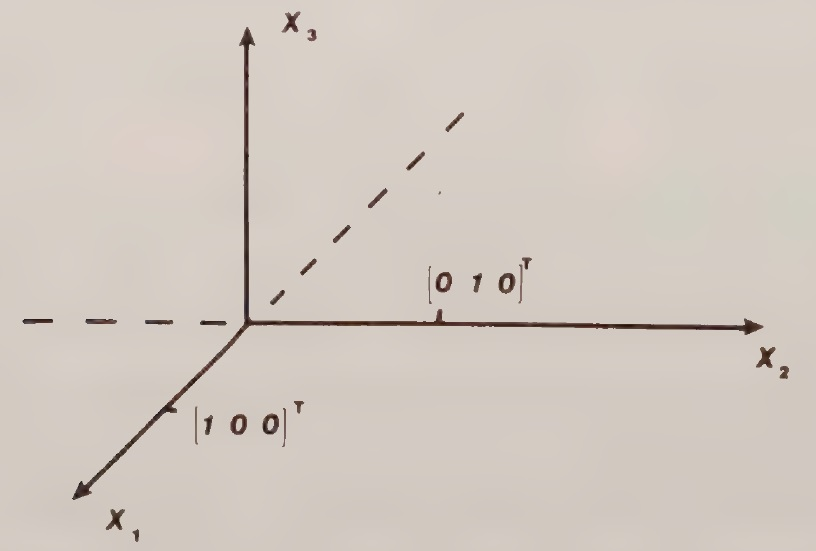
\includegraphics[width=0.58\linewidth,height=0.55\textheight,keepaspectratio]{figures/mp-2026/p068-hulls-example.jpg}
\end{frame}

% Source PDF page 069. Proposition 4's ray-only characterization was not
% sufficient for a convex cone and is corrected to nonnegative-combination
% closure; the remaining statements reproduce the source.
\begin{frame}{Affine \& Convex Sets}
  \footnotesize
  \begin{itemize}
    \item Proposition 1: For any nonempty set $S\subseteq\R^{n\times1}$,
      \begin{align*}
        S\subseteq X(S)\subseteq A(S)\subseteq L(S),\\
        S\subseteq X(S)\subseteq C(S)\subseteq L(S).
      \end{align*}
    \item Proposition 2: $S$ is a subspace of $\R^{n\times1}\Longleftrightarrow S=L(S)$
    \item Proposition 3: $S$ is an affine set $\Longleftrightarrow S=A(S)\Longleftrightarrow$ the line passing through any two distinct points in $S$ is a subset of $S$
    \item Proposition 4: $S$ is a convex cone $\Longleftrightarrow S=C(S)\Longleftrightarrow$ every nonnegative linear combination of points in $S$ belongs to $S$
    \item Proposition 5: $S$ is a convex set $\Longleftrightarrow S=X(S)\Longleftrightarrow$ the line segment connecting any two distinct points in $S$ is a subset of $S$
  \end{itemize}
\end{frame}

% Source PDF page 070
\begin{frame}{Affine \& Convex Sets}
  \small
  \begin{itemize}
    \item Proposition 6: A subset $S\subseteq\R^{n\times1}$ is affine $\Longleftrightarrow S-\vect{x}_0$ is a subspace of $\R^{n\times1}$, for every $\vect{x}_0\in S$
  \end{itemize}
  \begin{columns}[T,onlytextwidth]
    \begin{column}{0.52\textwidth}
      \begin{itemize}
        \item An affine set is just the translate of a subspace
        \item $\dim(S)=\dim(S-\vect{x}_0)$
        \item For any subset $T\subseteq\R^{n\times1}$, $\dim(T)=\dim(A(T))$
      \end{itemize}
    \end{column}
    \begin{column}{0.44\textwidth}
      \centering
      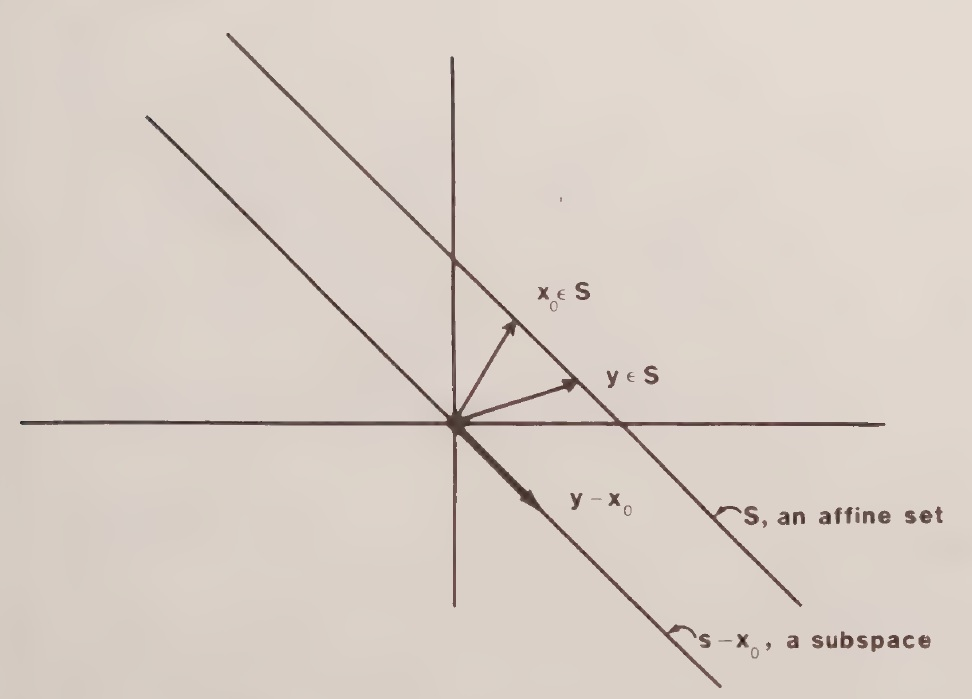
\includegraphics[width=\linewidth,height=0.48\textheight,keepaspectratio]{figures/mp-2026/p070-affine-translate.jpg}
    \end{column}
  \end{columns}
\end{frame}

\subsection{Hyperplanes, Polytopes, and Extreme Points}

% Source PDF page 071. The nonzero normal-vector condition is added because
% it is required in the definition of a hyperplane.
\begin{frame}{Affine \& Convex Sets}
  \small
  For $\vect{c}\ne\vect{0}$ and $\beta\in\R$:
  \begin{itemize}
    \item Hyperplane:
      \begin{equation*}H(\vect{c},\beta)=\{\vect{x}:\vect{c}^{\trans}\vect{x}=\beta\}\end{equation*}
    \item Upper half space:
      \begin{equation*}H^{+}(\vect{c},\beta)=\{\vect{x}:\vect{c}^{\trans}\vect{x}\ge\beta\}\end{equation*}
    \item Lower half space:
      \begin{equation*}H^{-}(\vect{c},\beta)=\{\vect{x}:\vect{c}^{\trans}\vect{x}\le\beta\}\end{equation*}
  \end{itemize}
  \centering
  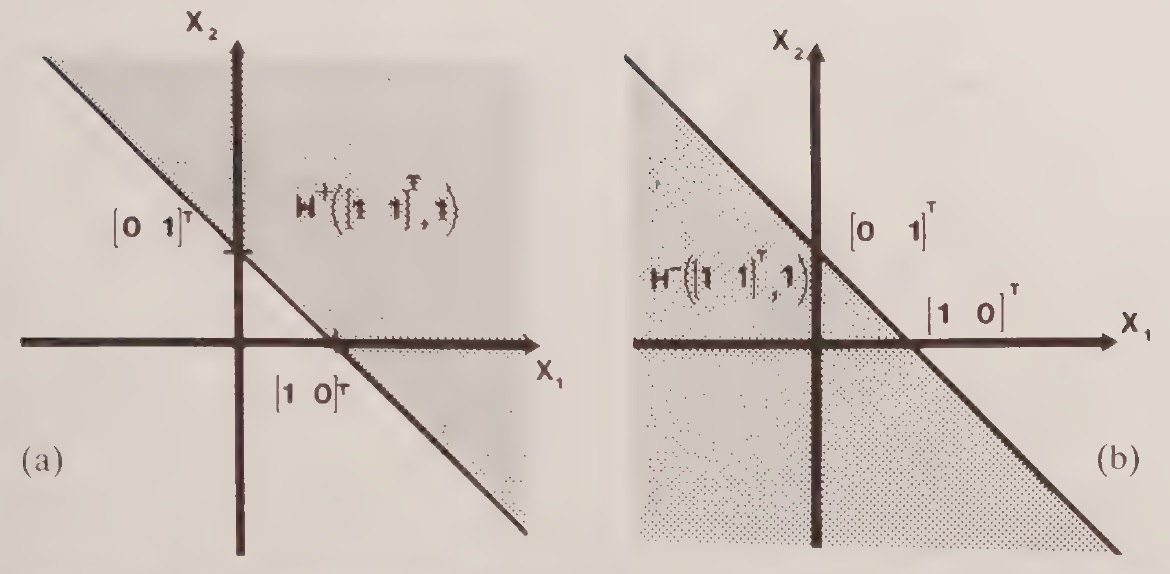
\includegraphics[width=0.38\linewidth,height=0.26\textheight,keepaspectratio]{figures/mp-2026/p071-hyperplane-halfspaces.jpg}
\end{frame}

% Source PDF page 072
\begin{frame}{Affine \& Convex Sets}
  \small
  \begin{columns}[T,onlytextwidth]
    \begin{column}{0.52\textwidth}
      \begin{itemize}
        \item Convex Polytope: $X(\{\vect{x}_1,\vect{x}_2,\ldots,\vect{x}_k\})$, $k<+\infty$
        \item Affinely Independent: $\{\vect{x}_0,\vect{x}_1,\ldots,\vect{x}_k\}$ is affinely independent $\Longleftrightarrow \{\vect{x}_1-\vect{x}_0,\vect{x}_2-\vect{x}_0,\ldots,\vect{x}_k-\vect{x}_0\}$ is linearly independent
        \item $k$-dimensional simplex: A convex polytope which is a convex hull of $k+1$ affinely independent vectors
      \end{itemize}
    \end{column}
    \begin{column}{0.44\textwidth}
      \centering
      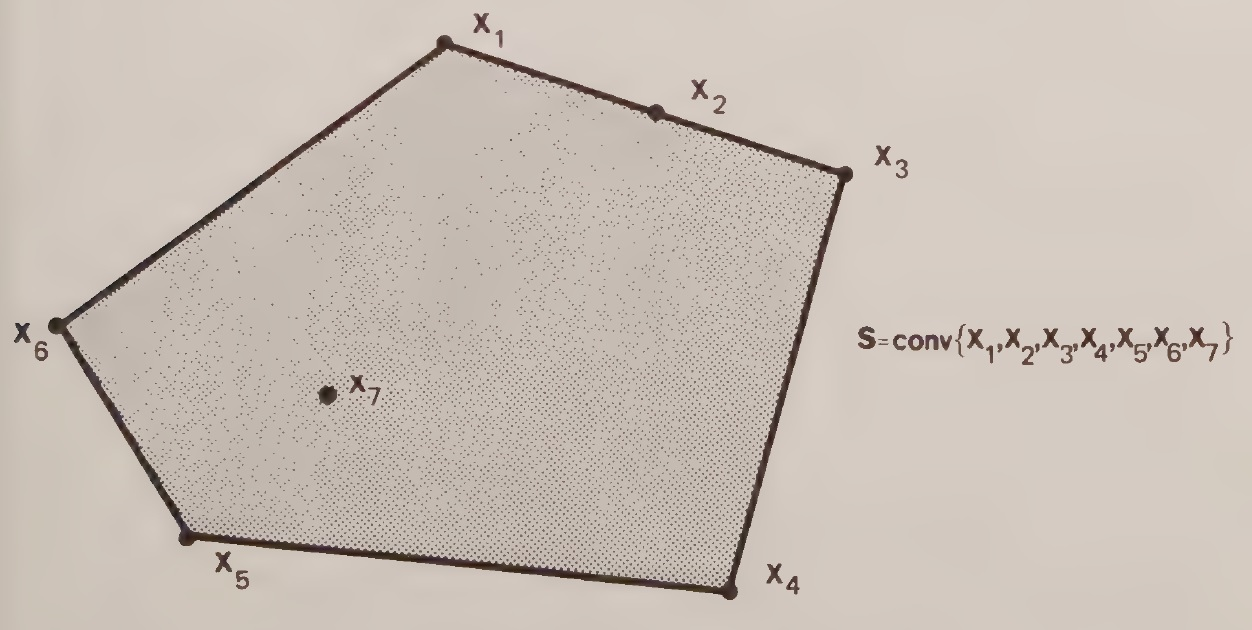
\includegraphics[width=\linewidth,height=0.52\textheight,keepaspectratio]{figures/mp-2026/p072-convex-polytope.jpg}
    \end{column}
  \end{columns}
\end{frame}

% Source PDF page 073
\begin{frame}{Affine \& Convex Sets}
  \centering
  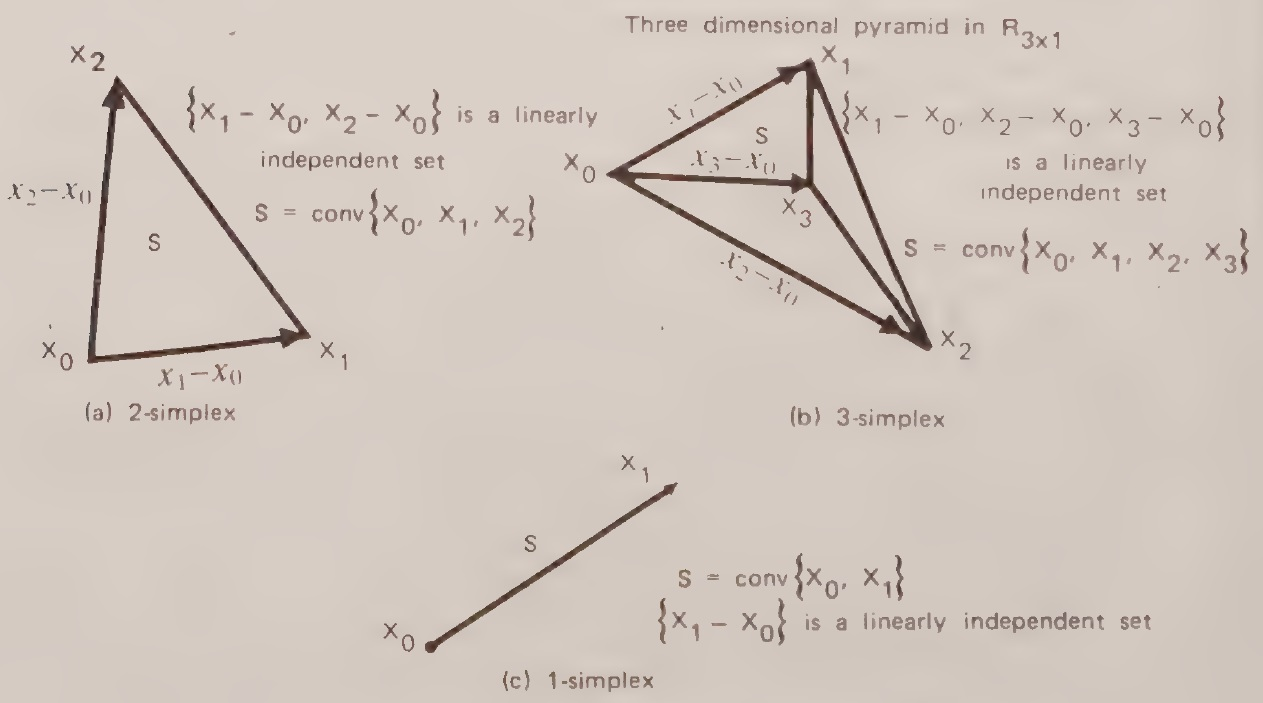
\includegraphics[width=0.76\linewidth,height=0.62\textheight,keepaspectratio]{figures/mp-2026/p073-simplex-examples.jpg}

  \smallskip
  Figure 1: (a) 2-simplex, (b) 3-simplex, (c) 1-simplex
\end{frame}

% Source PDF page 074. Source grammar ``pair of point'' corrected.
\begin{frame}{Affine \& Convex Sets}
  \small
  \begin{columns}[T,onlytextwidth]
    \begin{column}{0.57\textwidth}
      \begin{itemize}
        \item Extreme Point: $\vect{z}\in S$ (convex set) is an extreme point of $S$ $\Longleftrightarrow$ there does NOT exist distinct $\vect{x},\vect{y}\in S$ and $0<\alpha<1$ such that $\vect{z}=\alpha\vect{x}+(1-\alpha)\vect{y}$
        \item The vertices of any simplex are extreme points of the simplex
        \item The extreme points of a convex set $S$ are those NOT on the interior of any line segment connecting any other pair of points of $S$
      \end{itemize}
    \end{column}
    \begin{column}{0.39\textwidth}
      \centering
      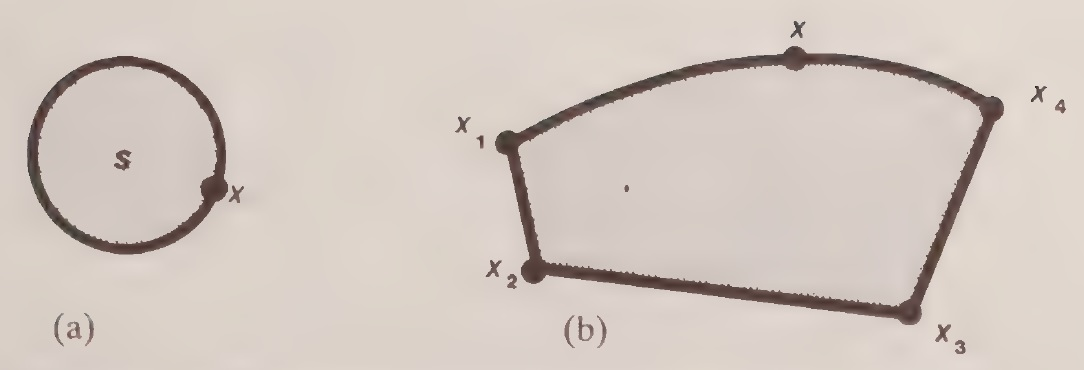
\includegraphics[width=\linewidth,height=0.43\textheight,keepaspectratio]{figures/mp-2026/p074-extreme-points.jpg}
    \end{column}
  \end{columns}
\end{frame}

\section{Linear Programming Problem}
\subsection{Feasible Polyhedra}

% Source PDF page 075
\begin{frame}{Linear Programming Problem}
  \begin{itemize}
    \item Original expression
      \begin{equation*}
        \min\ c_1x_1+\ldots+c_nx_n
      \end{equation*}
      subject to
      \begin{align*}
        a_{1,1}x_1+\ldots+a_{1,n}x_n&\le b_1,\\
        &\vdots\\
        a_{m,1}x_1+\ldots+a_{m,n}x_n&\le b_m,
      \end{align*}
      and
      \begin{equation*}
        \forall\ x_i\ge0.
      \end{equation*}
  \end{itemize}
\end{frame}

% Source PDF page 076
\begin{frame}{Linear Programming Problem}
  \begin{itemize}
    \item Equivalent expression:
      \begin{equation*}
        \min\ \vect{c}^{\trans}\vect{x}
      \end{equation*}
      subject to
      \begin{align*}
        A\vect{x}=A^{(1)}x_1+A^{(2)}x_2+\ldots+A^{(n)}x_n&\le\vect{b},\\
        \vect{x}&\ge\vect{0}.
      \end{align*}
    \item Set of feasible solutions: $F=\{\vect{x}:A\vect{x}\le\vect{b}\ \cap\ \vect{x}\ge\vect{0}\}$
  \end{itemize}
\end{frame}

% Source PDF page 077. ``half planes'' corrected to ``half spaces.''
\begin{frame}{Linear Programming Problem}
  \small
  \begin{itemize}
    \item Proposition 7: The set of feasible solution, $F$, to the linear programming problem is a convex set
    \item Proof: Let $\vect{x}_1,\vect{x}_2\in F$, $\alpha\in[0,1]$, check the convex combination $\vect{z}=\alpha\vect{x}_1+(1-\alpha)\vect{x}_2$. Does $\vect{z}\in F$?
    \item $F=\left(\bigcap_{i=1}^{m}\{\vect{x}:A_{(i)}\vect{x}\le b_i\}\right)
      \cap\left(\bigcap_{i=1}^{n}\{\vect{x}:x_i\ge0\}\right)$
    \item Convex polyhedron: Intersection of finite number of half spaces
    \item Convex polytope $\Longrightarrow$ Convex polyhedron; the converse does not hold in general
  \end{itemize}
\end{frame}

% Source PDF page 078
\begin{frame}{Linear Programming Problem}
  \begin{columns}[T,onlytextwidth]
    \begin{column}{0.49\textwidth}
      \centering
      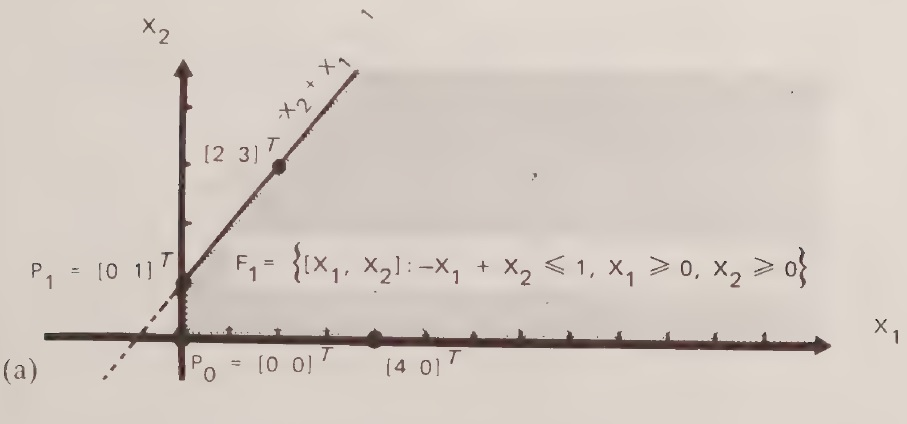
\includegraphics[width=\linewidth,height=0.53\textheight,keepaspectratio]{figures/mp-2026/p078-unbounded-polyhedron.jpg}\\
      \small (a) An unbounded convex polyhedron that is NOT a convex polytope
    \end{column}
    \begin{column}{0.49\textwidth}
      \centering
      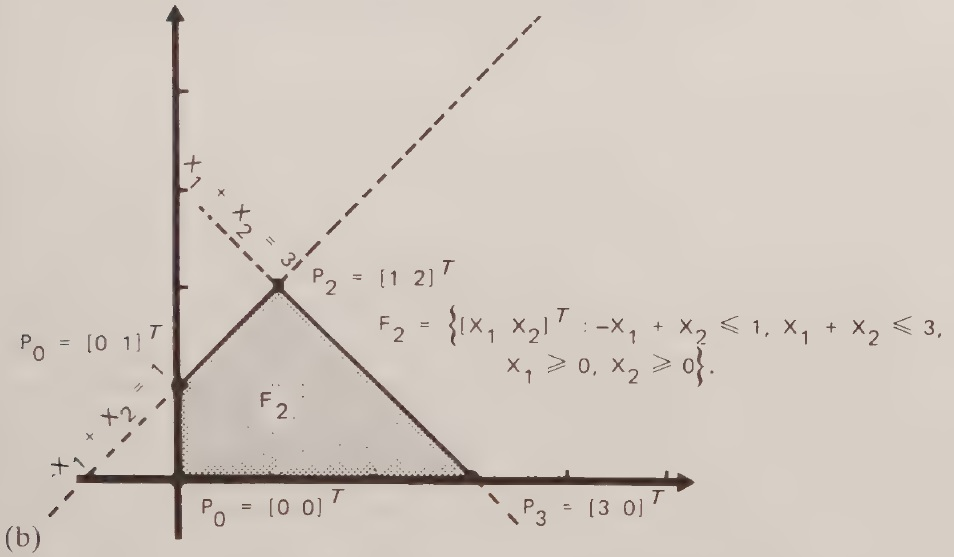
\includegraphics[width=\linewidth,height=0.53\textheight,keepaspectratio]{figures/mp-2026/p078-bounded-polytope.jpg}\\
      \small (b) A bounded convex polyhedron is a convex polytope
    \end{column}
  \end{columns}
\end{frame}

% Source PDF page 079. The source incorrectly required the finite point set
% to be the set of extreme points; the standard finite-generation statement
% below also covers polyhedra with lineality and no extreme points.
\begin{frame}{Linear Programming Problem}
  \small
  \begin{block}{Finite Basis Theorem}
    Let $F=\{\vect{x}\in\R^{n\times1}:A\vect{x}\le\vect{b}\}$ be a nonempty convex polyhedron. Then there exist finite sets $\{\vect{x}_1,\ldots,\vect{x}_d\}$ and $\{\vect{y}_1,\ldots,\vect{y}_{\ell}\}$ such that
    \begin{equation*}
      F=X(\{\vect{x}_1,\ldots,\vect{x}_d\})+C(\{\vect{y}_1,\ldots,\vect{y}_{\ell}\}),
    \end{equation*}
    i.e.,
    \begin{equation*}
      F=\left\{\sum_{i=1}^{d}\alpha_i\vect{x}_i+\sum_{j=1}^{\ell}\beta_j\vect{y}_j:
      \alpha_i\ge0,\ \beta_j\ge0,\ \sum_{i=1}^{d}\alpha_i=1\right\}.
    \end{equation*}
  \end{block}
\end{frame}

% Source PDF page 080
\begin{frame}{Linear Programming Problem}
  \centering
  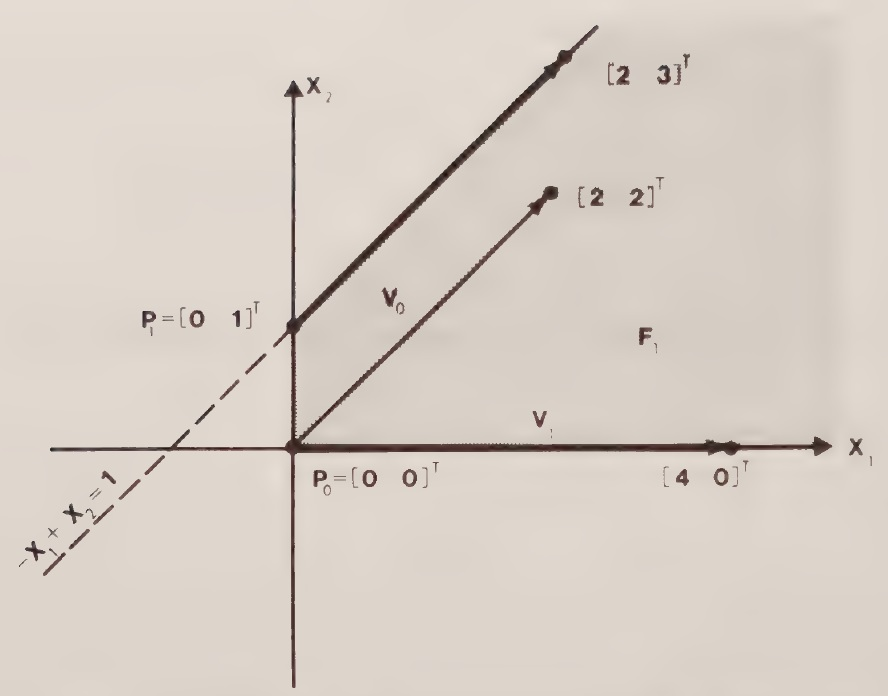
\includegraphics[width=0.56\linewidth,height=0.54\textheight,keepaspectratio]{figures/mp-2026/p080-finite-basis-decomposition.jpg}

  \footnotesize
  Figure 3: $F_2=X(\{\vect{p}_0,\vect{p}_1\})+C(\{\vect{v}_0,\vect{v}_1\})$, i.e., $F_2$ can be expressed as
  $\vect{x}=\alpha_0\vect{p}_0+\alpha_1\vect{p}_1+\beta_0\vect{v}_0+\beta_1\vect{v}_1$, where
  $\alpha_0\ge0$, $\alpha_1\ge0$, $\beta_0\ge0$, $\beta_1\ge0$ and $\alpha_0+\alpha_1=1$
\end{frame}

\end{document}
